\documentclass[a4paper, 11pt, twoside, fleqn]{memoir}

\usepackage{AOCDTF}

%--------------------------------------
%entrées du glossaire
%--------------------------------------

%création de macro-commande pour automatiser la rédaction de nouvelles entrées référencés dans le glossaire

\newglossaryentry{ex}{name={exemple}, description={définition de l'exemple d'entrée classique dans le glossaire}}
%--------------------------------------
%entrées des acronymes
%--------------------------------------

\newacronym{aocdtf}{AOCDTF}{Association Ouvrière des Compagnons du Devoir et du Tour de France}

\newacronym{ide}{IDE}{Environnement de Développement (Integrated Development Environment)}

\newacronym{isq}{ISQ}{International System of Quantities}

\newacronym{usi}{USI}{Unité du Système International}

\newacronym{si}{SI}{Système International}


\typemedia{paper} %choix screen ou paper pour les vidéos et schémas animés

\decoupagechapitre{1} %juste pour éviter les erreurs lors de la compilation des sous-programmations (passera en commentaire)
\marqueurchapitre

%lien d'édition des figures Tikz sur le site mathcha.io (rajouter le lien d'une modification effectuée sur la figure tikz avec le nom du modificateur car il n'y a qu'un lien par compte)

%lien mathcha Nom Prénom : 

%--------------------------------------
%corps du document
%--------------------------------------

\begin{document} %corps du document

	%--------------------------------------
	%espace de rédaction du document
	%--------------------------------------
	
\chapter{Exemples de tableaux\label{ann:exemples_tableaux}}	
	
Cette annexe regroupe des tableaux incluant toutes les notions évoquées dans le \superref{chap:tableaux}


\begin{exemple}{Tableau à la largeur relative, en-tête à doubles cellules, avec des listes du contenu mathématique}{}

Ce tableau à la largeur relative est codé dans l'environnement \mintinline{latex}{\begin{tableau}}, qui ne prend pas en compte les sauts de page. En l'insérant lui-même dans l'environnement \mintinline{latex}{\begin{table}}, celui-ci devient un élément \emph{flottant}, dont la disposition sur la page est pilotée par \LaTeX{}, qui pourra recevoir une légende et être référencé dans diverses listes.\\

Il met en évidence l'usage des types de colonnes \texttt{k}, qui insère un contenu automatiquement en mode mathématique aligné à droite. Sont aussi insérées des listes et des descriptions compactes dans une colonne de type \texttt{X}, en précisant l'instruction \mintinline{latex}{>{\compress}} juste avant la déclaration du type de colonne \texttt{X}.\\

L'en-tête est aussi scindée en deux lignes pour plus de clartés, avec l'instruction \mintinline{latex}{\cmidrule(lr){<première colonne>-<dernière colonne>}}, qui permet de séparer les lignes par des traits sous certaines cellules seulement.\\
Aussi, pour centrer l'en-tête de la colonnes \emph{Remarques}, il faut encadrer l'instruction \mintinline{latex}{\multirow{2}{*}{\thead{Remarque}}} avec l'instruction \mintinline{latex}{\multicolumn{1}{c}{\multirow{2}{*}{\thead{Remarque}}}} pour bien spécifier la variable optionnelle \texttt{c} prévue dans \mintinline{latex}{\multicolumn} et pas dans \mintinline{latex}{\multirow}.\\

\begin{minted}{latex}
\begin{table}[H]
\caption{Tableau à la largeur relative, en-tête à doubles cellules, avec des listes du contenu mathématique\label{tab:tableau_largeur_relative_en-tete_double_listes}}
\begin{tableau}{\textwidth}{l k l k >{\compress}X}
{\multicolumn{2}{c}{\thead{Grandeur}} & \multicolumn{2}{c}{\thead{Unité}} & \multicolumn{1}{c}{\multirow{2}{*}{\thead{Remarque}}} \\
\cmidrule(lr){1-2} \cmidrule(lr){3-4}
\thead[l]{Nom} & \multicolumn{1}{r}{\thead[r]{Symbole usuel}} & \thead[l]{Nom} & \multicolumn{1}{r}{\thead[r]{Symbole}} & }
Longueur 						& L, l					& Mètre			& \metre				& 
\begin{tabdescription}
\item[Item 1 :] un premier item\,;
\item[Item 2 :] un item avec une liste :
\begin{tabitemize}
\item un premier item\,;
\item un deuxième item\,;
\item un troisième item.
\end{tabitemize}
\end{tabdescription} \\
Largeur							& B, b					& 						&							& 
\begin{tabitemize}
\item un premier item\,;
\item un deuxième item\,;
\item un item avec une liste :
\begin{tabdescription}
\item[Item 1 :] un premier item\,;
\item[Item 2 :] un deuxième item.
\end{tabdescription}
\end{tabitemize}\\
Hauteur							& H, h					&						&							& Le symbole \(H\) est régulièrement utilisé pour désigner l'altitude. \\
\'Epaisseur						& d, \delta			& 						&							& \\
Rayon								& R, r					&						&							& \\
Distance radiale				& r_{Q}, \rho		&						&							& \\
Diamètre							& D, d					&						&							& \\
Longueur curviligne		& s						&						&							& \\
Distance							& d, r					& 						&							& \\
Rayon (vecteur)				& \mathbf{r}		&						&							& \\
\end{tableau}
\end{table}
\end{minted}

Cela produira :\\

\begin{table}[H]
\caption{Tableau à la largeur relative, en-tête à doubles cellules, avec des listes et du contenu mathématique\label{tab:tableau_largeur_relative_en-tete_double_listes}}
\begin{tableau}{\textwidth}{l k l k >{\compress}X}
{\multicolumn{2}{c}{\thead{Grandeur}} & \multicolumn{2}{c}{\thead{Unité}} & \multicolumn{1}{c}{\multirow{2}{*}{\thead{Remarque}}} \\
\cmidrule(lr){1-2} \cmidrule(lr){3-4}
\thead[l]{Nom} & \multicolumn{1}{r}{\thead[r]{Symbole usuel}} & \thead[l]{Nom} & \multicolumn{1}{r}{\thead[r]{Symbole}} & }
Longueur 						& L, l					& Mètre			& \metre				& 
\begin{tabdescription}
\item[Item 1 :] un premier item\,;
\item[Item 2 :] un item avec une liste :
\begin{tabitemize}
\item un premier item\,;
\item un deuxième item\,;
\item un troisième item.
\end{tabitemize}
\end{tabdescription} \\
Largeur							& B, b					& 						&							& 
\begin{tabitemize}
\item un premier item\,;
\item un deuxième item\,;
\item un item avec une liste :
\begin{tabdescription}
\item[Item 1 :] un premier item\,;
\item[Item 2 :] un deuxième item.
\end{tabdescription}
\end{tabitemize}\\
Hauteur							& H, h					&						&							& Le symbole \(H\) est régulièrement utilisé pour désigner l'altitude. \\
\'Epaisseur						& d, \delta			& 						&							& \\
Rayon								& R, r					&						&							& \\
Distance radiale				& r_{Q}, \rho		&						&							& \\
Diamètre							& D, d					&						&							& \\
Longueur curviligne		& s						&						&							& \\
Distance							& d, r					& 						&							& \\
Rayon (vecteur)				& \mathbf{r}		&						&							& \\
\end{tableau}
\end{table}
\end{exemple}

\begin{exemple}{Tableau à la largeur relative sur plusieurs pages, avec des notes en bas de tableaux et des titres de colonnes obliques}{tableau_largeur_relative_plusieurs_pages_notes_obliques}

Ce tableau à la largeur relative met en évidence les sauts de pages et l'usage de l'environnement \mintinline{latex}{\begin{longtableau}}. Il inclus également des notes en bas tableau avec les environnements \mintinline{latex}{\begin{TableNotes}} et \mintinline{latex}{\begin{ThreePartTable}}, ainsi que l'instruction \mintinline{latex}{\tnote{<numéro de la note>}}. Il faut bien veiller à appeler l'environnement \mintinline{latex}{\begin{TableNotes}} \emph{avant} de rédiger le tableau dans l'environnement \mintinline{latex}{\begin{ThreePartTable}} et de l'appeler avec l'option \mintinline{latex}{[\notetableau]} en option de l'environnement \mintinline{latex}{\begin{longtableau}}.\\

Les en-têtes obliques sont appelés avec l'instruction \mintinline{latex}{\mcrot{<nombre de colonnes à cheval>}{<alignement horizontal du texte>}{<angle>}{<contenu de la cellule>}}.\\

On remarque aussi que les titres de colonnes inclus dans l'instruction \mintinline{latex}{\thead{<titre de la colonne>}} peut contenir un retour à la ligne afin d'éviter que celui-ci ne soit trop et ne déstructure le tableau. Pour structurer et aérer le tableau, on utilise ici l'instruction \mintinline{latex}{\middashrule}. 

\begin{minted}{latex}
    	\begin{TableNotes}
    \item[1] une première notre en bas de tableau\,;
    \item[2] une deuxième notre en bas de tableau.
  \end{TableNotes}
    \begin{ThreePartTable}
	\begin{longtableau}[t]{\linewidth}{c CCCCCCCCCCCCCCCC}{17}{Tableau à la largeur relative sur plusieurs pages, avec des notes en bas de tableaux et des titres de colonnes obliques}{
\multirow[c]{2}{*}{\thead{Section des\\conducteurs\\(\si{\square\milli\meter})\tnote{1}}}	& \multicolumn{16}{l}{\thead{Courant assigné (\si{\ampere})\tnote{2}}} \\
\cmidrule(lr){2-17} 
& \mcrot{1}{l}{60}{1} 	& \mcrot{1}{l}{60}{2} & \mcrot{1}{l}{60}{3}	& \mcrot{1}{l}{60}{4} & \mcrot{1}{l}{60}{6} & \mcrot{1}{l}{60}{10} & \mcrot{1}{l}{60}{16} & \mcrot{1}{l}{60}{20} &\mcrot{1}{l}{60}{25} & \mcrot{1}{l}{60}{32} & \mcrot{1}{l}{60}{40} & \mcrot{1}{l}{60}{50} & \mcrot{1}{l}{60}{63} & \mcrot{1}{l}{60}{80} & \mcrot{1}{l}{60}{100} & \mcrot{1}{l}{60}{125}}[\notetableau]
1,5		&	429 &	21&	143 &	107 &	71 & 43 & 27 & 21 & 17 & 13 & 11 & 9 & 7 & 5 & 4 & 3 \\
\middashrule
2,5		&	714	 &	357		&	238		&	179		&	119	&	71 & 45 & 36 & 29 &	22 & 18 & 14 & 11 &	9 &	7 & 6 \\
\middashrule
4 & &	571 &	381 &	286 &	190	&	114	&	71	&	57	&	46	&	36	&	29	&	23 &	18 &	14 &	11		&	9 \\
\middashrule
6 & &	857 &	571 &	429 &	286	&	171	&	107	&	86 &	69 &	54 &	43 &	34		&	27		&	21		&	17		&	14 \\
\middashrule
10 & & &	952 & 714 & 476 & 286 & 179 & 143 & 114 & 89 & 71 & 57 & 45 & 36 & 29 & 23 \\
\middashrule
16 & &	 &	 &	 & 762 & 457 & 286 & 229 & 183 & 143 & 114 & 91 & 73 & 57 & 46 & 37 \\
\middashrule
25 & &	 &	 &	 & & 714 & 446 & 357 & 286 & 223 & 179 & 143 & 113 & 89 & 71 & 57 \\
\middashrule
35 & & & & & && 625 & 500 & 400 & 313 & 250 & 200 & 159 & 125 & 100 & 80 \\
\middashrule
50 & & & & & & & & 679 & 543 & 424 & 339 & 271 & 215 & 170 & 136 & 109 \\
\middashrule
1,5		&	429 &	21&	143 &	107 &	71 & 43 & 27 & 21 & 17 & 13 & 11 & 9 & 7 & 5 & 4 & 3 \\
\middashrule
2,5		&	714	 &	357		&	238		&	179		&	119	&	71 & 45 & 36 & 29 &	22 & 18 & 14 & 11 &	9 &	7 & 6 \\
\middashrule
4 & &	571 &	381 &	286 &	190	&	114	&	71	&	57	&	46	&	36	&	29	&	23 &	18 &	14 &	11		&	9 \\
\middashrule
6 & &	857 &	571 &	429 &	286	&	171	&	107	&	86 &	69 &	54 &	43 &	34		&	27		&	21		&	17		&	14 \\
\middashrule
10 & & &	952 & 714 & 476 & 286 & 179 & 143 & 114 & 89 & 71 & 57 & 45 & 36 & 29 & 23 \\
\middashrule
16 & &	 &	 &	 & 762 & 457 & 286 & 229 & 183 & 143 & 114 & 91 & 73 & 57 & 46 & 37 \\
\middashrule
25 & &	 &	 &	 & & 714 & 446 & 357 & 286 & 223 & 179 & 143 & 113 & 89 & 71 & 57 \\
\middashrule
35 & & & & & && 625 & 500 & 400 & 313 & 250 & 200 & 159 & 125 & 100 & 80 \\
\middashrule
50 & & & & & & & & 679 & 543 & 424 & 339 & 271 & 215 & 170 & 136 & 109 \\
\middashrule
1,5		&	429 &	21&	143 &	107 &	71 & 43 & 27 & 21 & 17 & 13 & 11 & 9 & 7 & 5 & 4 & 3 \\
\middashrule
2,5		&	714	 &	357		&	238		&	179		&	119	&	71 & 45 & 36 & 29 &	22 & 18 & 14 & 11 &	9 &	7 & 6 \\
\middashrule
4 & &	571 &	381 &	286 &	190	&	114	&	71	&	57	&	46	&	36	&	29	&	23 &	18 &	14 &	11		&	9 \\
\middashrule
6 & &	857 &	571 &	429 &	286	&	171	&	107	&	86 &	69 &	54 &	43 &	34		&	27		&	21		&	17		&	14 \\
\middashrule
10 & & &	952 & 714 & 476 & 286 & 179 & 143 & 114 & 89 & 71 & 57 & 45 & 36 & 29 & 23 \\
\middashrule
16 & &	 &	 &	 & 762 & 457 & 286 & 229 & 183 & 143 & 114 & 91 & 73 & 57 & 46 & 37 \\
\middashrule
25 & &	 &	 &	 & & 714 & 446 & 357 & 286 & 223 & 179 & 143 & 113 & 89 & 71 & 57 \\
\middashrule
35 & & & & & && 625 & 500 & 400 & 313 & 250 & 200 & 159 & 125 & 100 & 80 \\
\middashrule
50 & & & & & & & & 679 & 543 & 424 & 339 & 271 & 215 & 170 & 136 & 109 \\
\end{longtableau}
    \end{ThreePartTable}
\end{minted}

Cela produira (tableau situé en dehors de l'environnement exemple pour des raisons de compatibilité) :\\


\end{exemple}

    	\begin{TableNotes}
    \item[1] une première note en bas de tableau\,;
    \item[2] une deuxième note en bas de tableau.
  \end{TableNotes}
    \begin{ThreePartTable}
	\begin{longtableau}[t]{\linewidth}{c CCCCCCCCCCCCCCCC}{17}{Tableau à la largeur relative sur plusieurs pages, avec des notes en bas de tableaux et des titres de colonnes obliques}{
\multirow[c]{2}{*}{\thead{Section des\\conducteurs\\(\si{\square\milli\meter})\tnote{1}}}	& \multicolumn{16}{l}{\thead{Courant assigné (\si{\ampere})\tnote{2}}} \\
\cmidrule(lr){2-17} 
& \mcrot{1}{l}{60}{1} 	& \mcrot{1}{l}{60}{2} & \mcrot{1}{l}{60}{3}	& \mcrot{1}{l}{60}{4} & \mcrot{1}{l}{60}{6} & \mcrot{1}{l}{60}{10} & \mcrot{1}{l}{60}{16} & \mcrot{1}{l}{60}{20} &\mcrot{1}{l}{60}{25} & \mcrot{1}{l}{60}{32} & \mcrot{1}{l}{60}{40} & \mcrot{1}{l}{60}{50} & \mcrot{1}{l}{60}{63} & \mcrot{1}{l}{60}{80} & \mcrot{1}{l}{60}{100} & \mcrot{1}{l}{60}{125}}[\notetableau]
1,5		&	429		&	214		&	143		&	107		&	71		&	43		&	27		&	21		&	17		&	13		&	11		&	9		&	7		&	5		&	4		&	3 \\
\middashrule
2,5		&	714		&	357		&	238		&	179		&	119	&	71		&	45		&	36		&	29		&	22		&	18		&	14		&	11		&	9		&	7		&	6 \\
\middashrule
4			&				&	571		&	381		&	286		&	190	&	114	&	71		&	57		&	46		&	36		&	29		&	23		&	18		&	14		&	11		&	9 \\
\middashrule
6			&				&	857		&	571		&	429		&	286	&	171	&	107	&	86		&	69		&	54		&	43		&	34		&	27		&	21		&	17		&	14 \\
\middashrule
10			&				&				&	952		&	714		&	476	&	286	&	179	&	143	&	114	&	89		&	71		&	57		&	45		&	36		&	29		&	23 \\
\middashrule
16			&				&				&				&				&	762	&	457	&	286	&	229	&	183	&	143	&	114	&	91		&	73		&	57		&	46		&	37 \\
\middashrule
25			&				&				&				&				&			&	714	&	446	&	357	&	286	&	223	&	179	&	143	&	113	&	89		&	71		&	57 \\
\middashrule
35			&				&				&				&				&			&			&	625	&	500	&	400	&	313	&	250	&	200	&	159	&	125	&	100	&	80 \\
\middashrule
50			&				&				&				&				&			&			&			&	679	&	543	&	424	&	339	&	271	&	215	&	170	&	136	&	109 \\
\middashrule
1,5		&	429		&	214		&	143		&	107		&	71		&	43		&	27		&	21		&	17		&	13		&	11		&	9		&	7		&	5		&	4		&	3 \\
\middashrule
2,5		&	714		&	357		&	238		&	179		&	119	&	71		&	45		&	36		&	29		&	22		&	18		&	14		&	11		&	9		&	7		&	6 \\
\middashrule
4			&				&	571		&	381		&	286		&	190	&	114	&	71		&	57		&	46		&	36		&	29		&	23		&	18		&	14		&	11		&	9 \\
\middashrule
6			&				&	857		&	571		&	429		&	286	&	171	&	107	&	86		&	69		&	54		&	43		&	34		&	27		&	21		&	17		&	14 \\
\middashrule
10			&				&				&	952		&	714		&	476	&	286	&	179	&	143	&	114	&	89		&	71		&	57		&	45		&	36		&	29		&	23 \\
\middashrule
16			&				&				&				&				&	762	&	457	&	286	&	229	&	183	&	143	&	114	&	91		&	73		&	57		&	46		&	37 \\
\middashrule
25			&				&				&				&				&			&	714	&	446	&	357	&	286	&	223	&	179	&	143	&	113	&	89		&	71		&	57 \\
\middashrule
35			&				&				&				&				&			&			&	625	&	500	&	400	&	313	&	250	&	200	&	159	&	125	&	100	&	80 \\
\middashrule
50			&				&				&				&				&			&			&			&	679	&	543	&	424	&	339	&	271	&	215	&	170	&	136	&	109 \\
\middashrule
1,5		&	429		&	214		&	143		&	107		&	71		&	43		&	27		&	21		&	17		&	13		&	11		&	9		&	7		&	5		&	4		&	3 \\
\middashrule
2,5		&	714		&	357		&	238		&	179		&	119	&	71		&	45		&	36		&	29		&	22		&	18		&	14		&	11		&	9		&	7		&	6 \\
\middashrule
4			&				&	571		&	381		&	286		&	190	&	114	&	71		&	57		&	46		&	36		&	29		&	23		&	18		&	14		&	11		&	9 \\
\middashrule
6			&				&	857		&	571		&	429		&	286	&	171	&	107	&	86		&	69		&	54		&	43		&	34		&	27		&	21		&	17		&	14 \\
\middashrule
10			&				&				&	952		&	714		&	476	&	286	&	179	&	143	&	114	&	89		&	71		&	57		&	45		&	36		&	29		&	23 \\
\middashrule
16			&				&				&				&				&	762	&	457	&	286	&	229	&	183	&	143	&	114	&	91		&	73		&	57		&	46		&	37 \\
\middashrule
25			&				&				&				&				&			&	714	&	446	&	357	&	286	&	223	&	179	&	143	&	113	&	89		&	71		&	57 \\
\middashrule
35			&				&				&				&				&			&			&	625	&	500	&	400	&	313	&	250	&	200	&	159	&	125	&	100	&	80 \\
\middashrule
50			&				&				&				&				&			&			&			&	679	&	543	&	424	&	339	&	271	&	215	&	170	&	136	&	109 \\
\end{longtableau}
    \end{ThreePartTable}


\begin{exemple}{Tableau à la largeur relative en paysage sur plusieurs pages, avec insertion de figures}{}

Ce tableau explicite l'insertion de figures dans un tableau, \emph{toujours} alignées sur le haut de la cellule avec l'instruction \mintinline{latex}{\adjustbox{valign=t}{\includegraphics[width=<largeur>]{<chemin d'accès de l'image>}}}.

\begin{minted}{latex}
\begin{landscape}
\begin{longtableau}{\linewidth}{p{0.3cm} c X p{0.3cm} c X p{0.3cm} c X}{9}{Tableau à la largeur relative en paysage sur plusieurs pages, avec insertion de figures}
{\multicolumn{3}{c}{\thead{Protection contre les corps solides}}	& \multicolumn{3}{c}{\thead{Lettre additionnelle\\Contact direct avec les parties dangereuses}}	& \multicolumn{3}{c}{\thead{Protection contre les liquides}}}[\notetableau]
0 		& 									& Aucune protection	&	&	&	& 0 	&	&	Aucune protection \\
\addlinespace
1 		& \adjustbox{valign=t}{
\includegraphics[width=2cm]{fig_image.png}} & Protégé contre les corps solides \(\diameter \geq \SI{50}{\milli\meter}\)  	&	A & \adjustbox{valign=t}{
\includegraphics[width=2cm]{fig_image.png}}	&	Le dos de la main reste éloigné des parties dangereuses.	& 1 & 	\adjustbox{valign=t}{
\includegraphics[width=2cm]{fig_image.png}}	&	Protégé contre les chutes verticales de gouttes d'eau (condensation) \\
\addlinespace
2 		& 	\adjustbox{valign=t}{
\includegraphics[width=2cm]{fig_image_a.png}} & Protégé contre les corps solides \(\diameter \geq \SI{12,5}{\milli\meter}\)  	& B	& \adjustbox{valign=t}{
\includegraphics[width=2cm]{fig_image_a.png}}	&	L'introduction d'un doigt ne permet pas de toucher les parties dangereuses. & 2 & 	\adjustbox{valign=t}{
\includegraphics[width=2cm]{fig_image_a.png}}	&	Protégé contre les chutes de gouttes d'eau jusqu'à 15° de la verticale \\
\addlinespace
3 		& 	\adjustbox{valign=t}{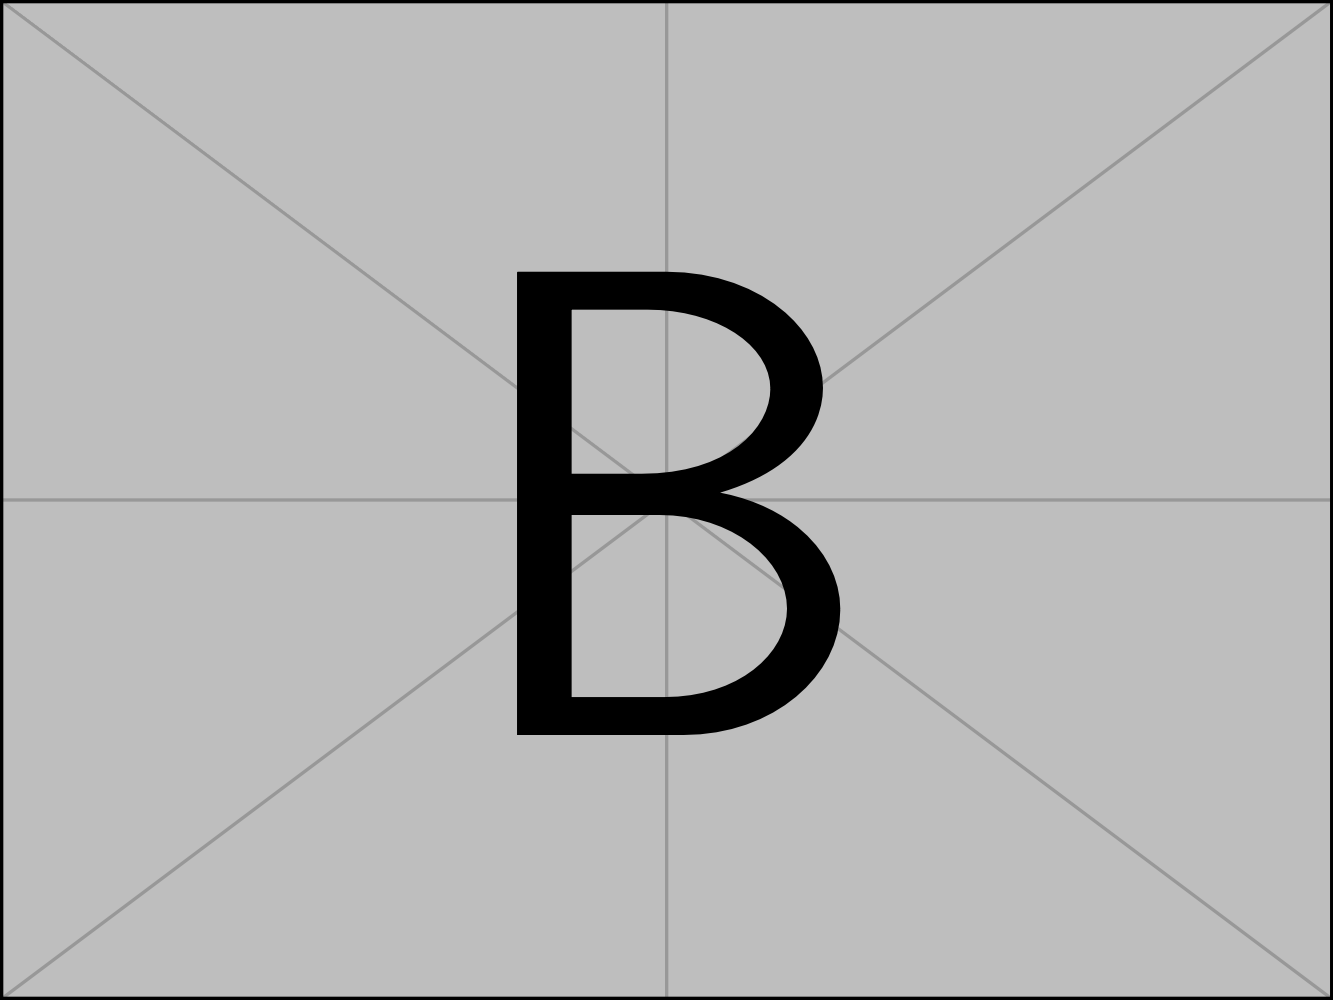
\includegraphics[width=2cm]{fig_image_b.png}} & Protégé contre les corps solides \(\diameter \geq \SI{2,5}{\milli\meter}\)  	& C	& \adjustbox{valign=t}{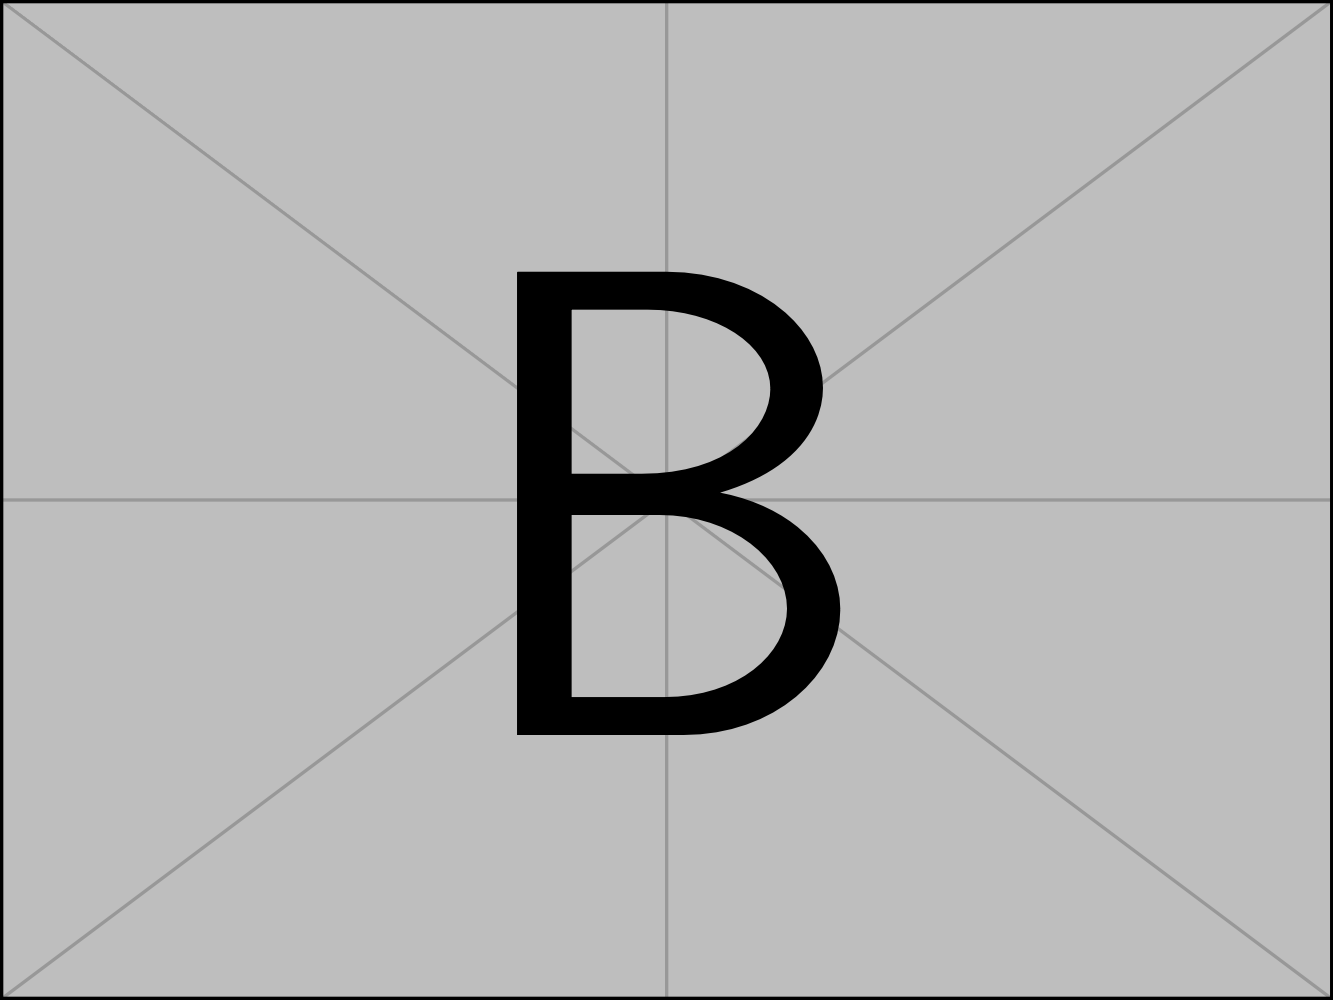
\includegraphics[width=2cm]{fig_image_b.png}}	&	L'introduction d'un outil ne permet pas de toucher les parties dangereuses. & 3 & 	\adjustbox{valign=t}{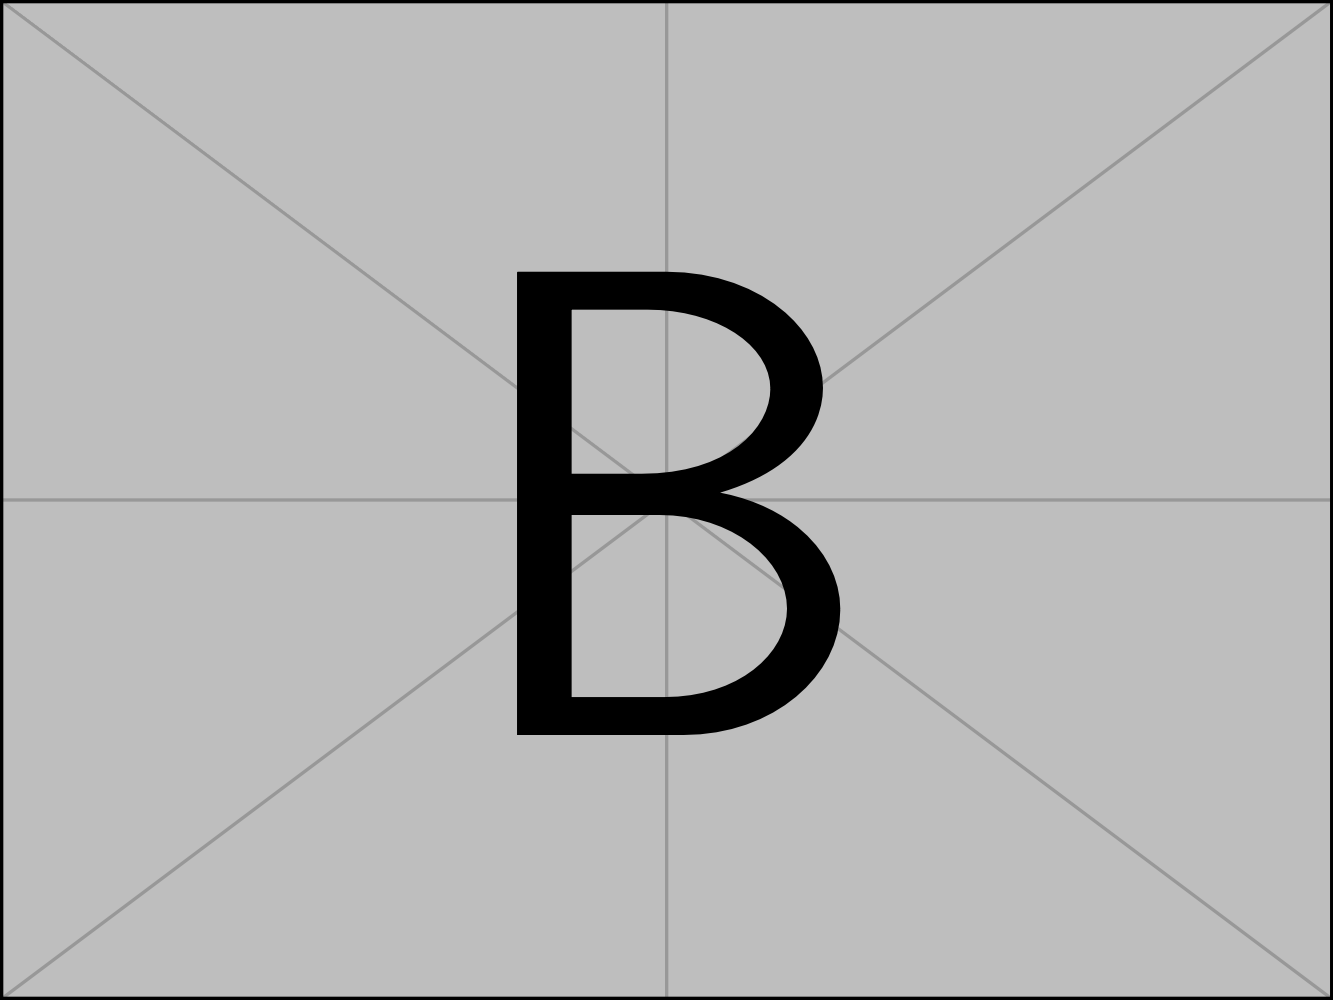
\includegraphics[width=2cm]{fig_image_b.png}}	&	Protégé contre l'eau de pluie jusqu'à 60° de la verticale \\
\addlinespace
4 		& 	\adjustbox{valign=t}{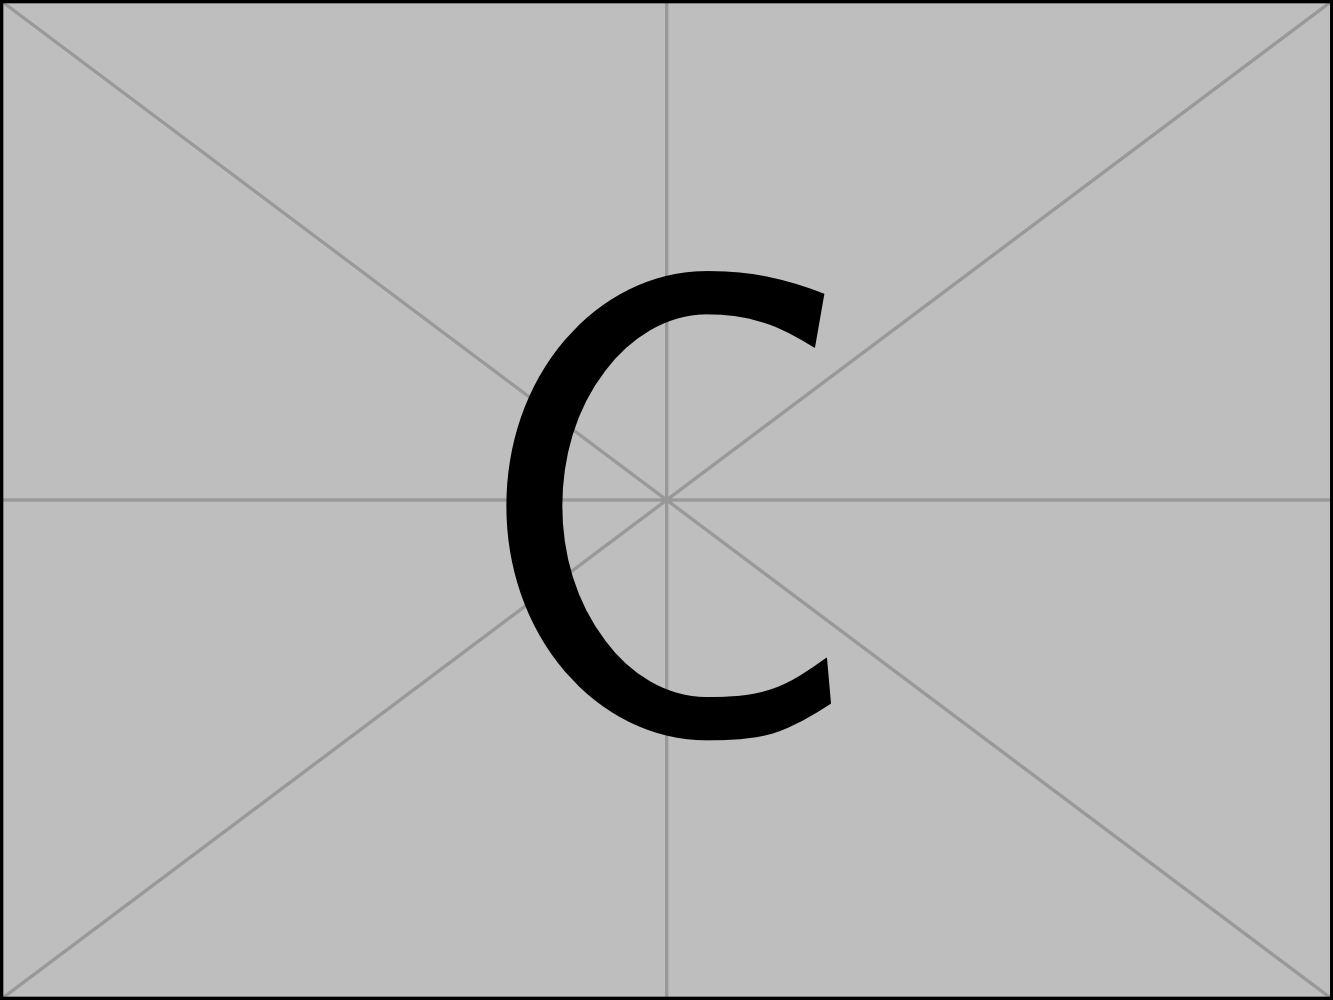
\includegraphics[width=2cm]{fig_image_c.png}} & Protégé contre les corps solides \(\diameter \geq \SI{1}{\milli\meter}\)  	& D	& \adjustbox{valign=t}{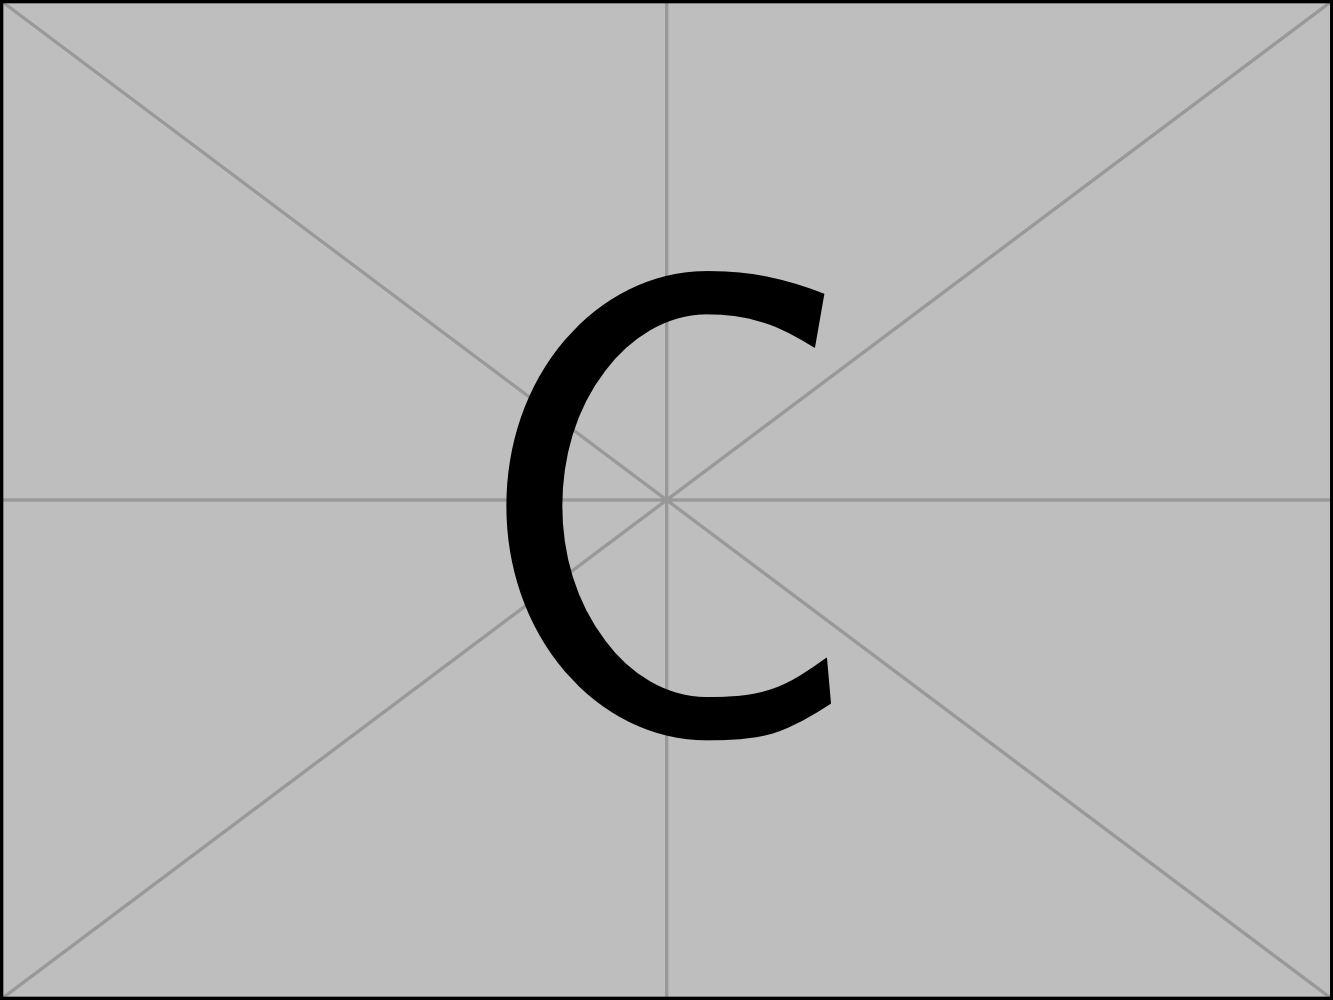
\includegraphics[width=2cm]{fig_image_c.png}}	&	L'introduction d'un outil fin ne permet pas de toucher les parties dangereuses. & 4 & 	\adjustbox{valign=t}{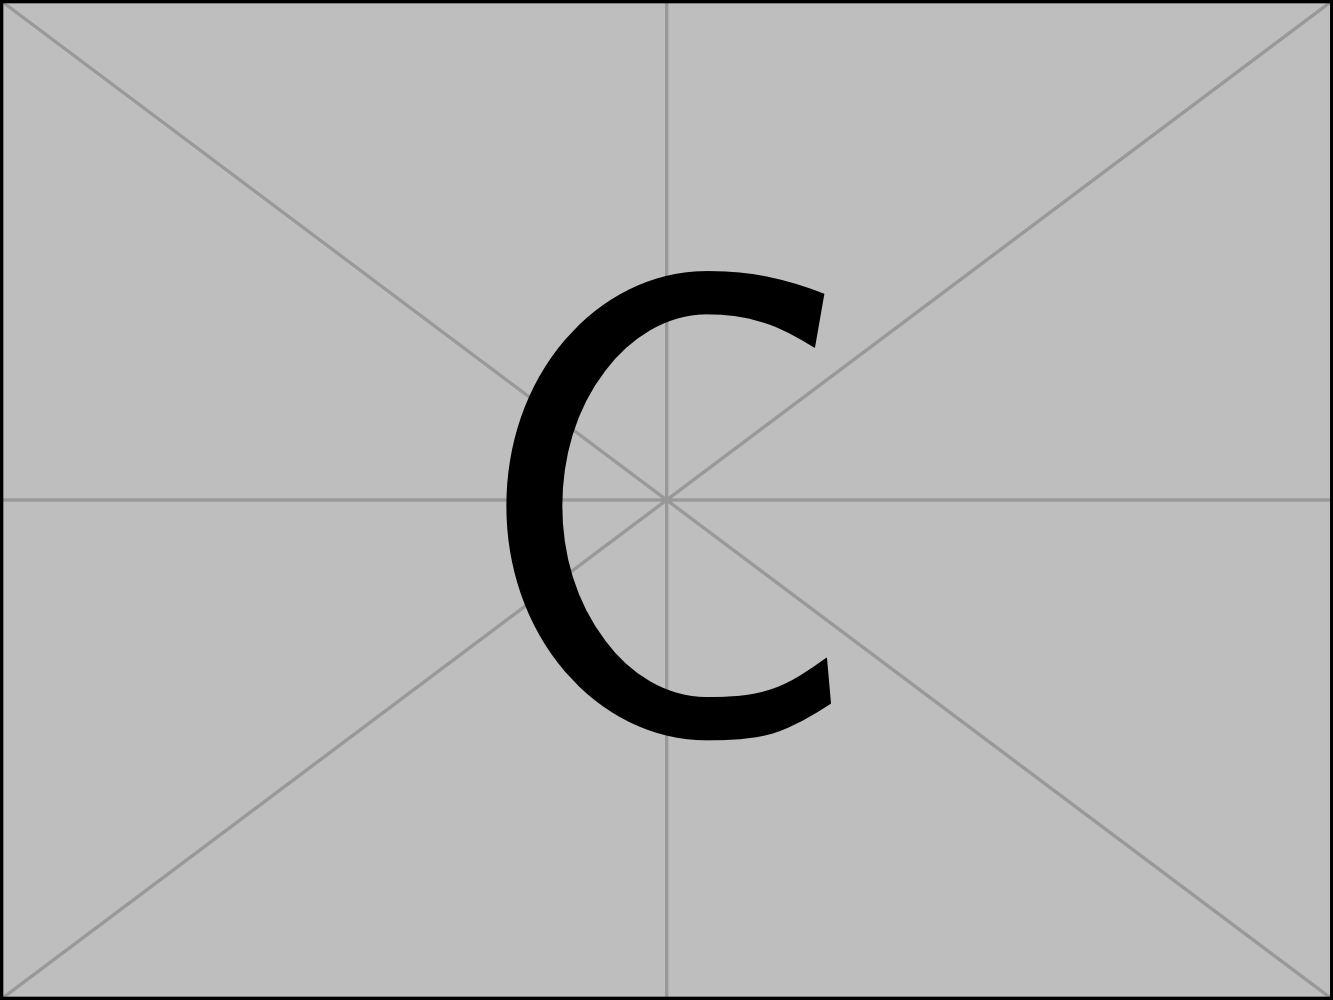
\includegraphics[width=2cm]{fig_image_c.png}}	&	Protégé contre les projections d'eau dans toutes les directions \\
\addlinespace
5 		& 	\adjustbox{valign=t}{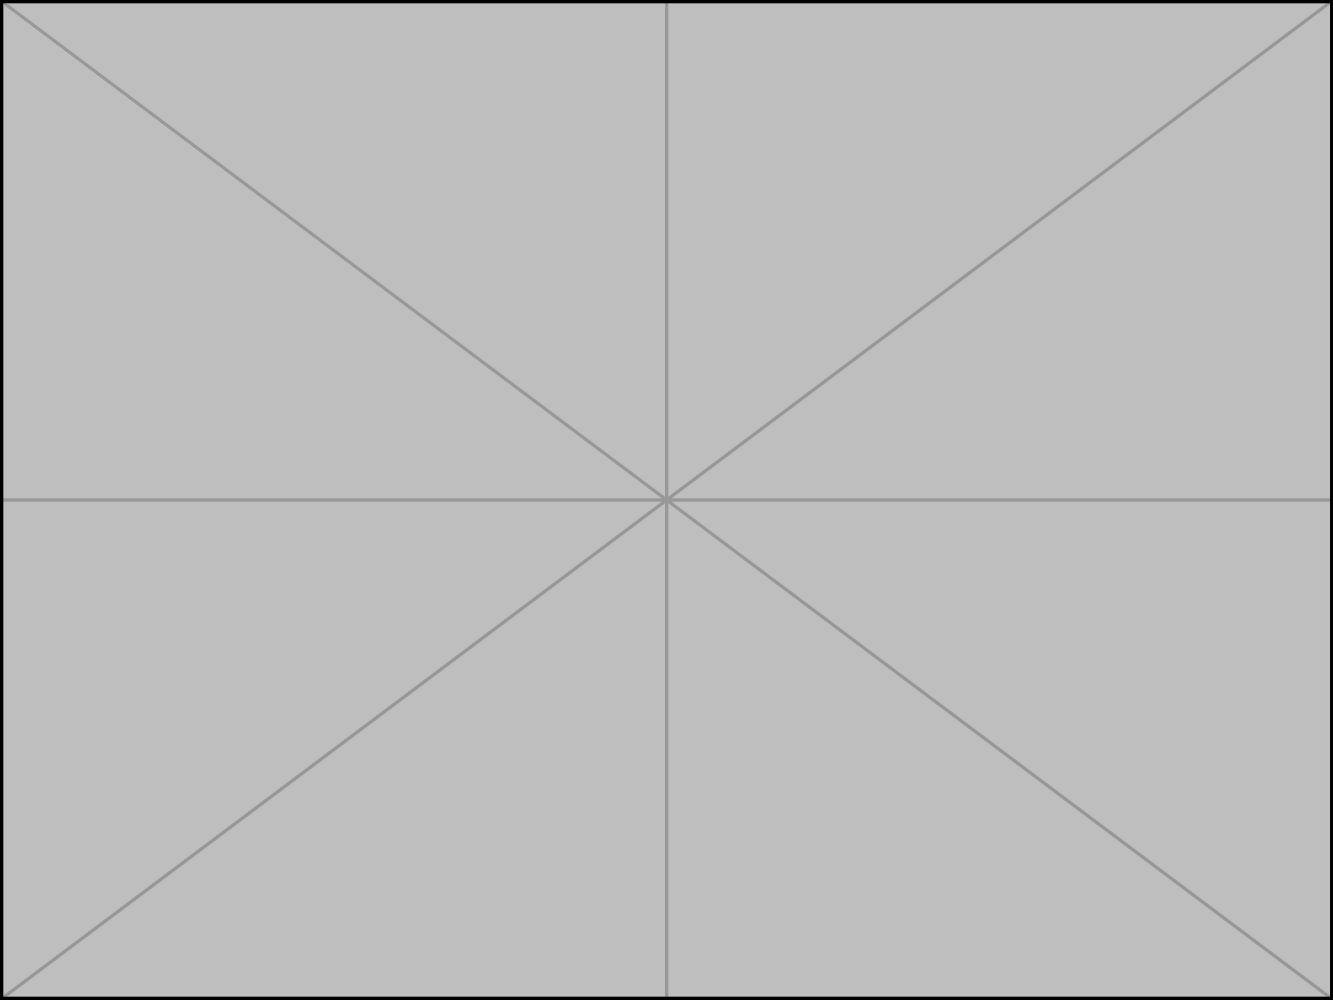
\includegraphics[width=2cm]{fig_image_vide.png}} & Protégé contre la poussière (pas de dépot nuisible)  	& 	& & & 5 & 	\adjustbox{valign=t}{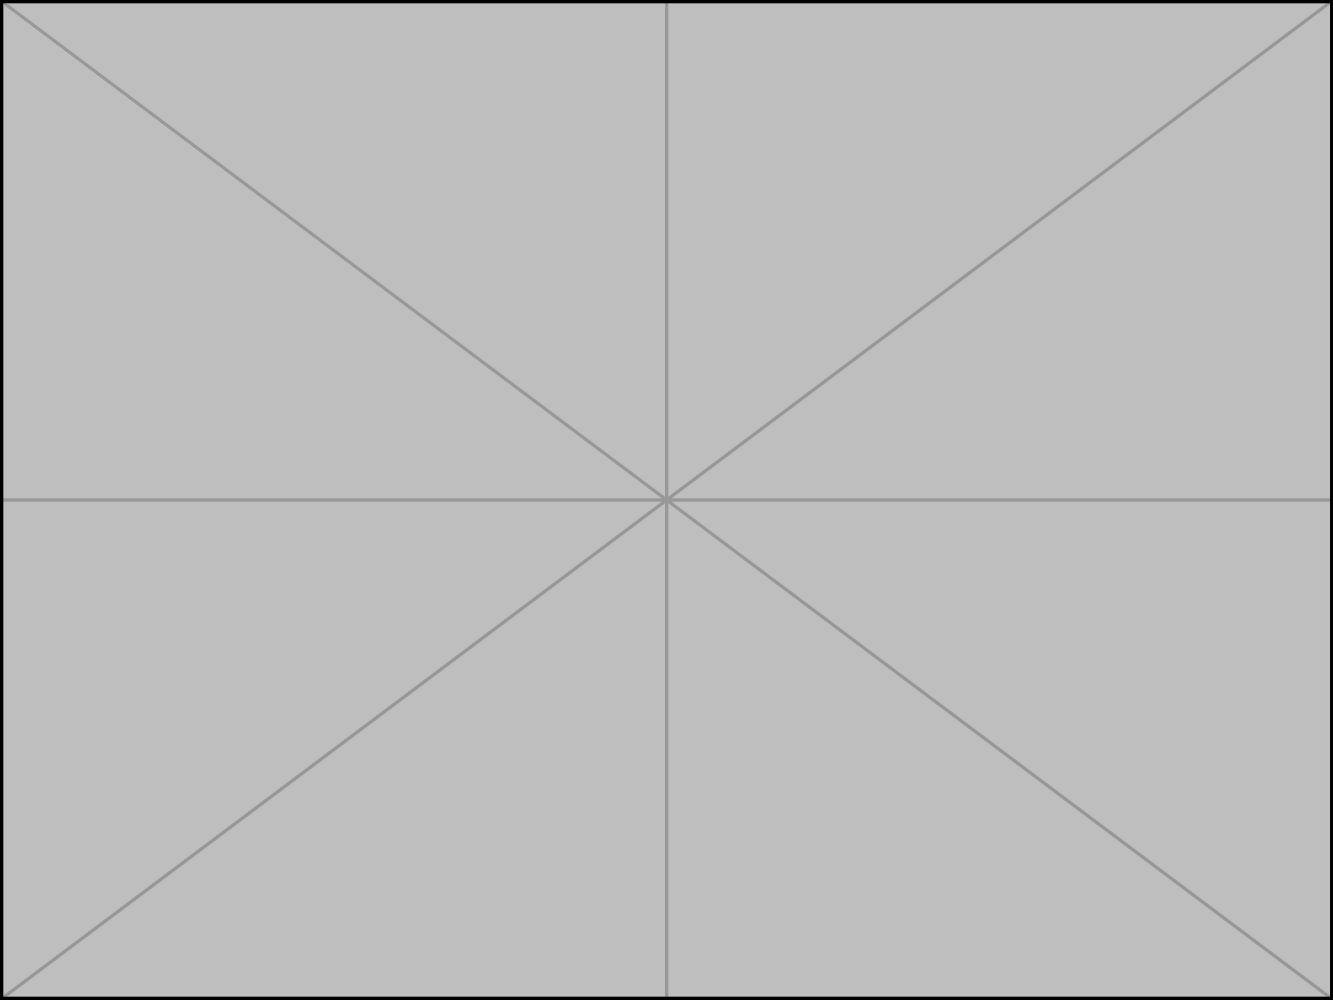
\includegraphics[width=2cm]{fig_image_vide.png}}	&	Protégé contre les jets d'eau dans toutes les directions à la lance \\
\addlinespace
6 		& \adjustbox{valign=t}{
\includegraphics[width=2cm]{fig_image.png}} & Totalement protégé contre la poussière 	& 	& & & 6 & 	\adjustbox{valign=t}{
\includegraphics[width=2cm]{fig_image.png}}	&	Protégé contre les projections d'eau assimilables aux paquets de mer \\
\addlinespace
 		&  & 	& 	& & & 7 & 	\adjustbox{valign=t}{
\includegraphics[width=2cm]{fig_image_a.png}}	&	Protégé contre les effets d'une immersion temporaire dans l'eau \\
 		\addlinespace
		&  & 	& 	& & & 8 & 	\adjustbox{valign=t}{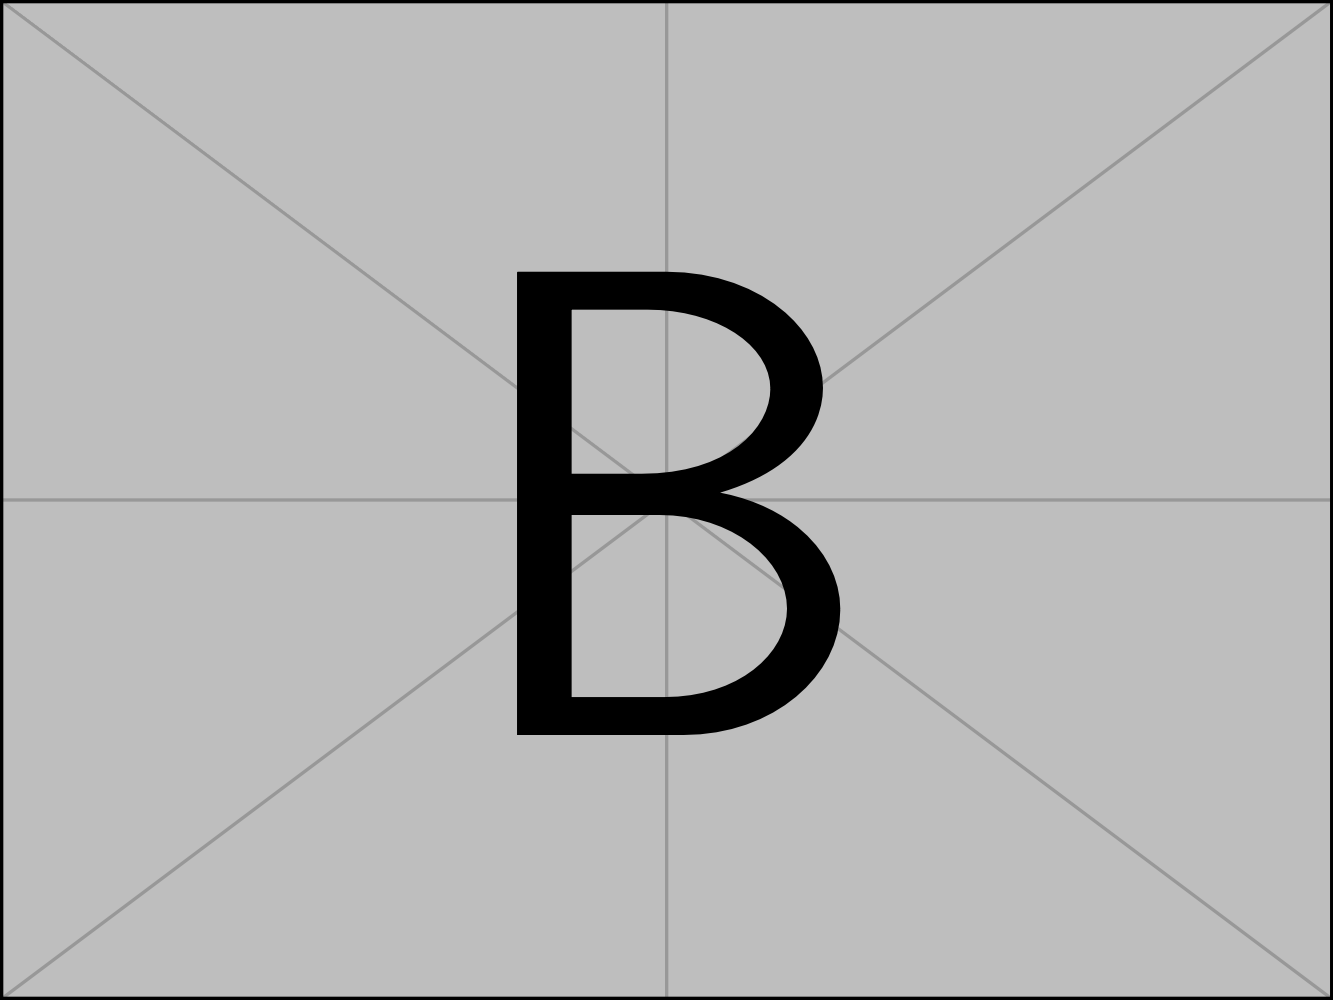
\includegraphics[width=2cm]{fig_image_b.png}}	&	Protégé contre les effets d'une immersion prolongée dans l'eau dans des conditions spécifiées \\
		\addlinespace
		&  & 	& 	& & & 9 & 	&	Protégé contre les jets d'eau haute pression et haute température mais pas nécessairement submersible \\
\end{longtableau}	
\end{landscape}
\end{minted}

Cela produira (tableau situé en dehors de l'environnement exemple pour des raisons de compatibilité) :\\


\end{exemple}


\begin{landscape}
    	\begin{TableNotes}
    \item[3] une troisième note en bas de tableau\,;
    \item[1000] une millième note en bas de tableau.
  \end{TableNotes}
  \begin{ThreePartTable}
\begin{longtableau}{\linewidth}{p{0.3cm} c X p{0.3cm} c X p{0.3cm} c X}{9}{Tableau à la largeur relative en paysage sur plusieurs pages, avec insertion de figures}
{\multicolumn{3}{c}{\thead{Protection contre les corps solides}}	& \multicolumn{3}{c}{\thead{Lettre additionnelle\\Contact direct avec les parties dangereuses}}	& \multicolumn{3}{c}{\thead{Protection contre les liquides}}}[\notetableau]
0 		& 									& Aucune protection	&	&	&	& 0 	&	&	Aucune protection \\
\addlinespace
1 		& \adjustbox{valign=t}{
\includegraphics[width=2cm]{fig_image.png}} & Protégé contre les corps solides \(\diameter \geq \SI{50}{\milli\meter}\)\tnote{3}  	&	A & \adjustbox{valign=t}{
\includegraphics[width=2cm]{fig_image.png}}	&	Le dos de la main reste éloigné des parties dangereuses.	& 1 & 	\adjustbox{valign=t}{
\includegraphics[width=2cm]{fig_image.png}}	&	Protégé contre les chutes verticales de gouttes d'eau (condensation) \\
\addlinespace
2 		& 	\adjustbox{valign=t}{
\includegraphics[width=2cm]{fig_image_a.png}} & Protégé contre les corps solides \(\diameter \geq \SI{12,5}{\milli\meter}\)  	& B	& \adjustbox{valign=t}{
\includegraphics[width=2cm]{fig_image_a.png}}	&	L'introduction d'un doigt ne permet pas de toucher les parties dangereuses. & 2 & 	\adjustbox{valign=t}{
\includegraphics[width=2cm]{fig_image_a.png}}	&	Protégé contre les chutes de gouttes d'eau jusqu'à 15° de la verticale \\
\addlinespace
3 		& 	\adjustbox{valign=t}{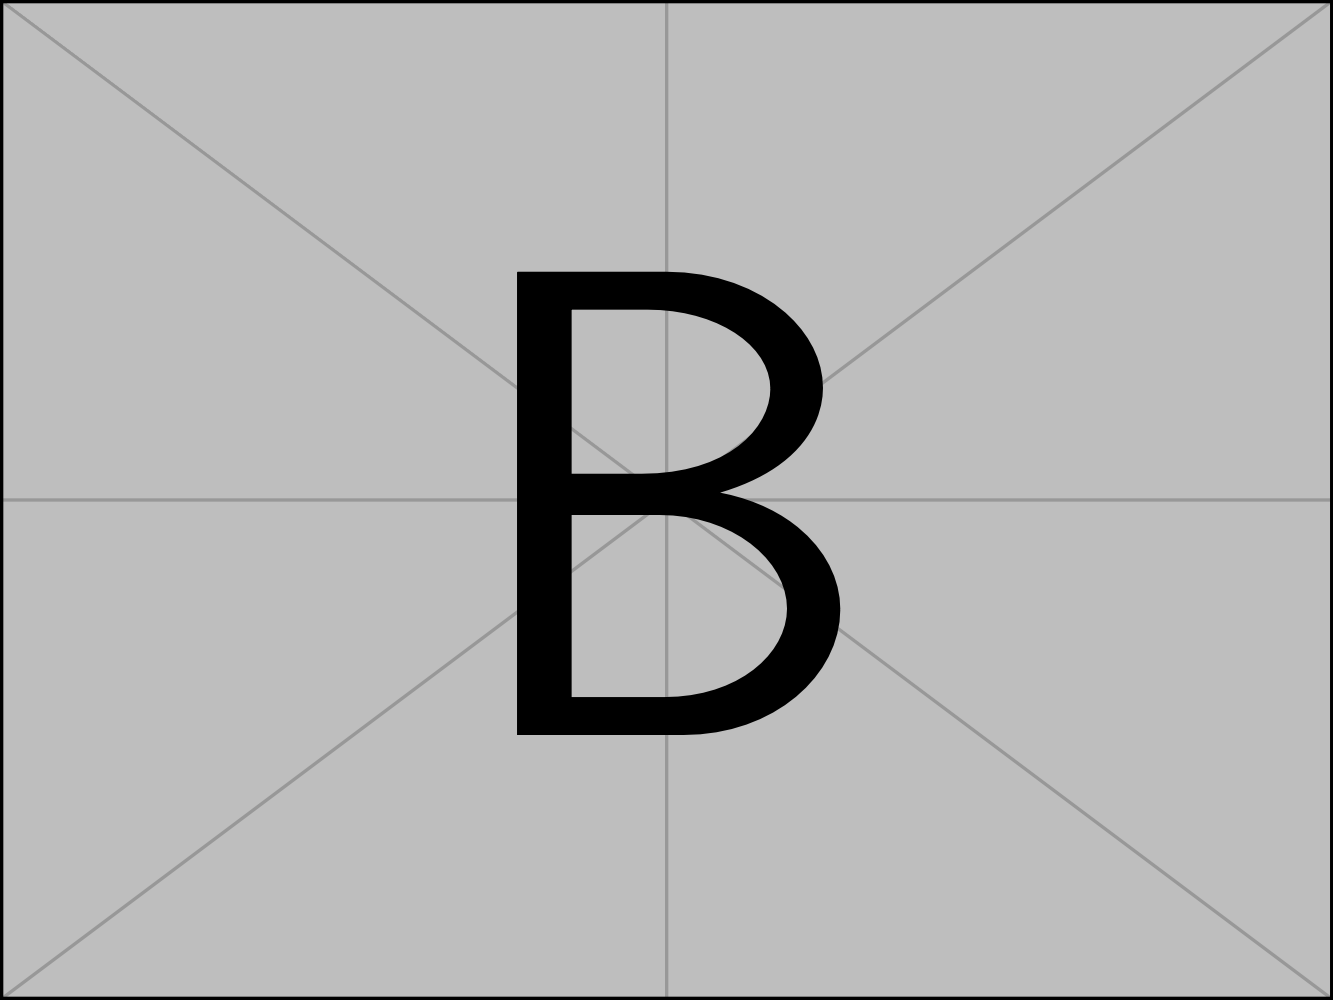
\includegraphics[width=2cm]{fig_image_b.png}} & Protégé contre les corps solides \(\diameter \geq \SI{2,5}{\milli\meter}\)\tnote{1000} 	& C	& \adjustbox{valign=t}{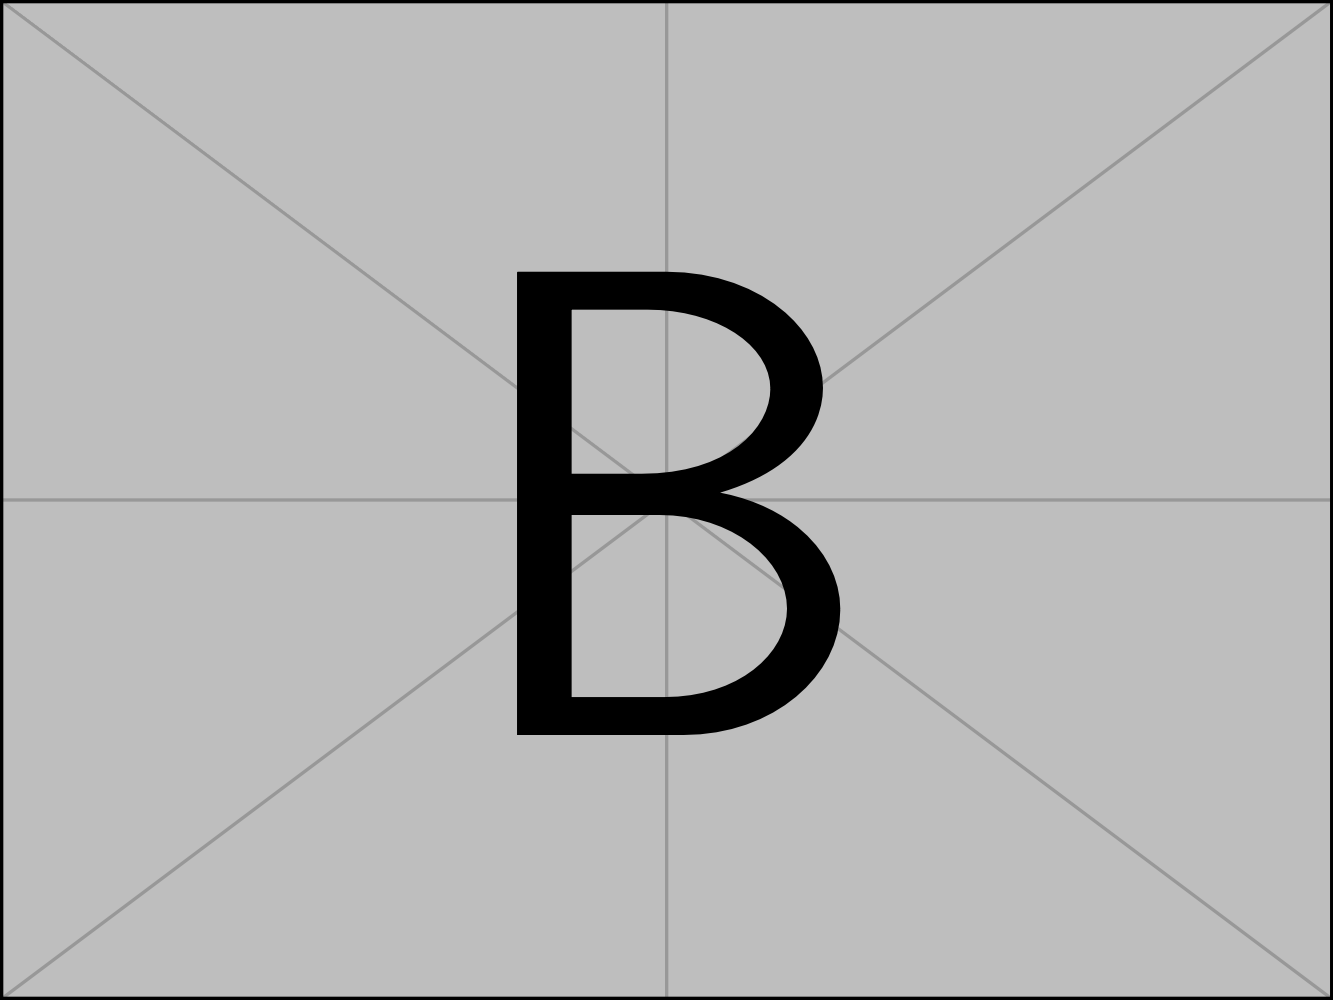
\includegraphics[width=2cm]{fig_image_b.png}}	&	L'introduction d'un outil ne permet pas de toucher les parties dangereuses. & 3 & 	\adjustbox{valign=t}{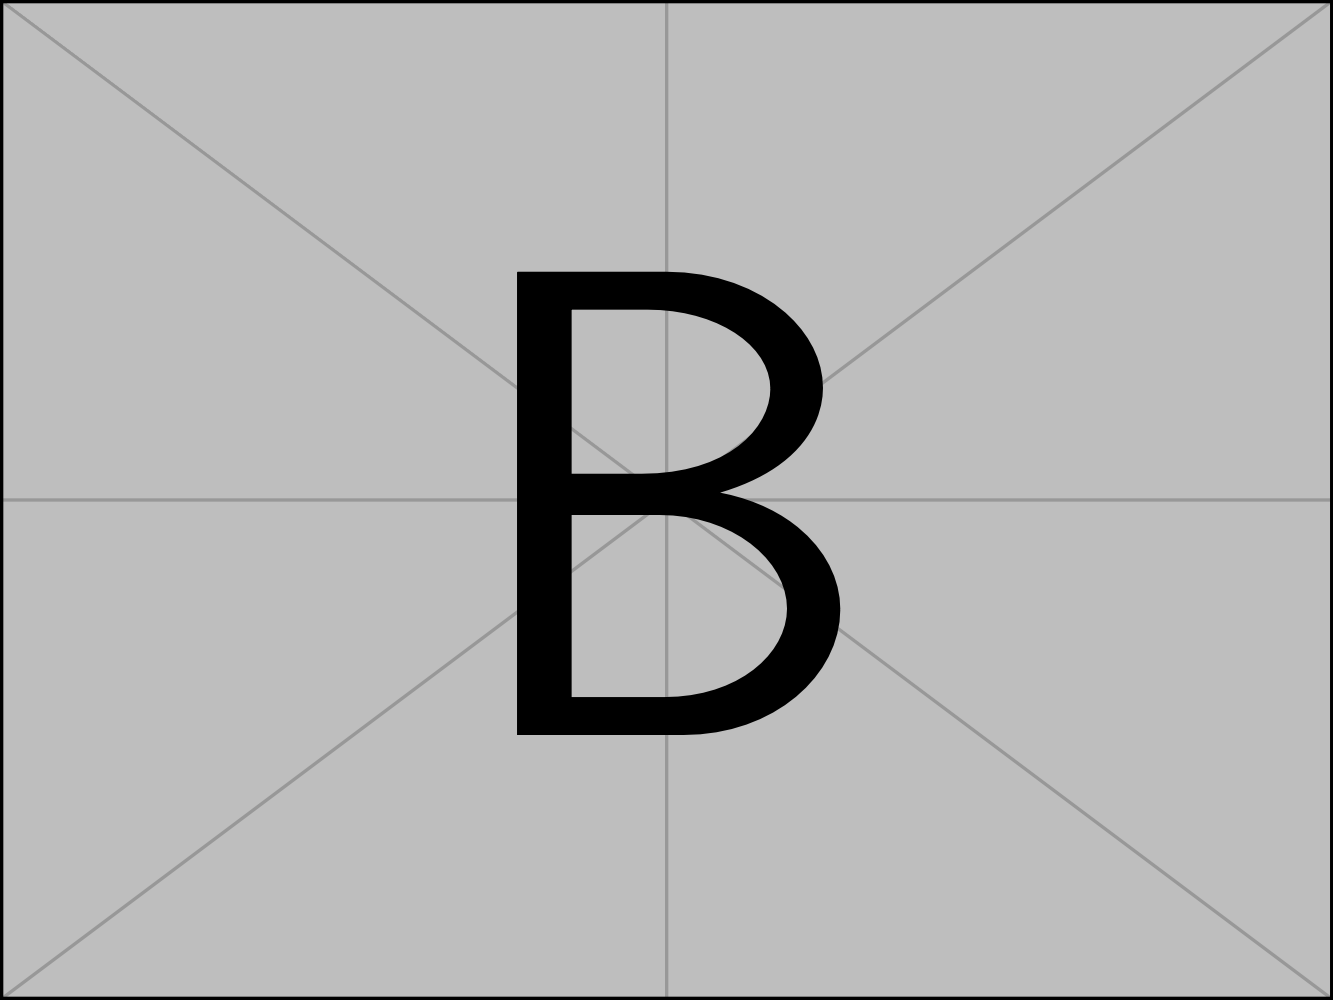
\includegraphics[width=2cm]{fig_image_b.png}}	&	Protégé contre l'eau de pluie jusqu'à 60° de la verticale \\
\addlinespace
4 		& 	\adjustbox{valign=t}{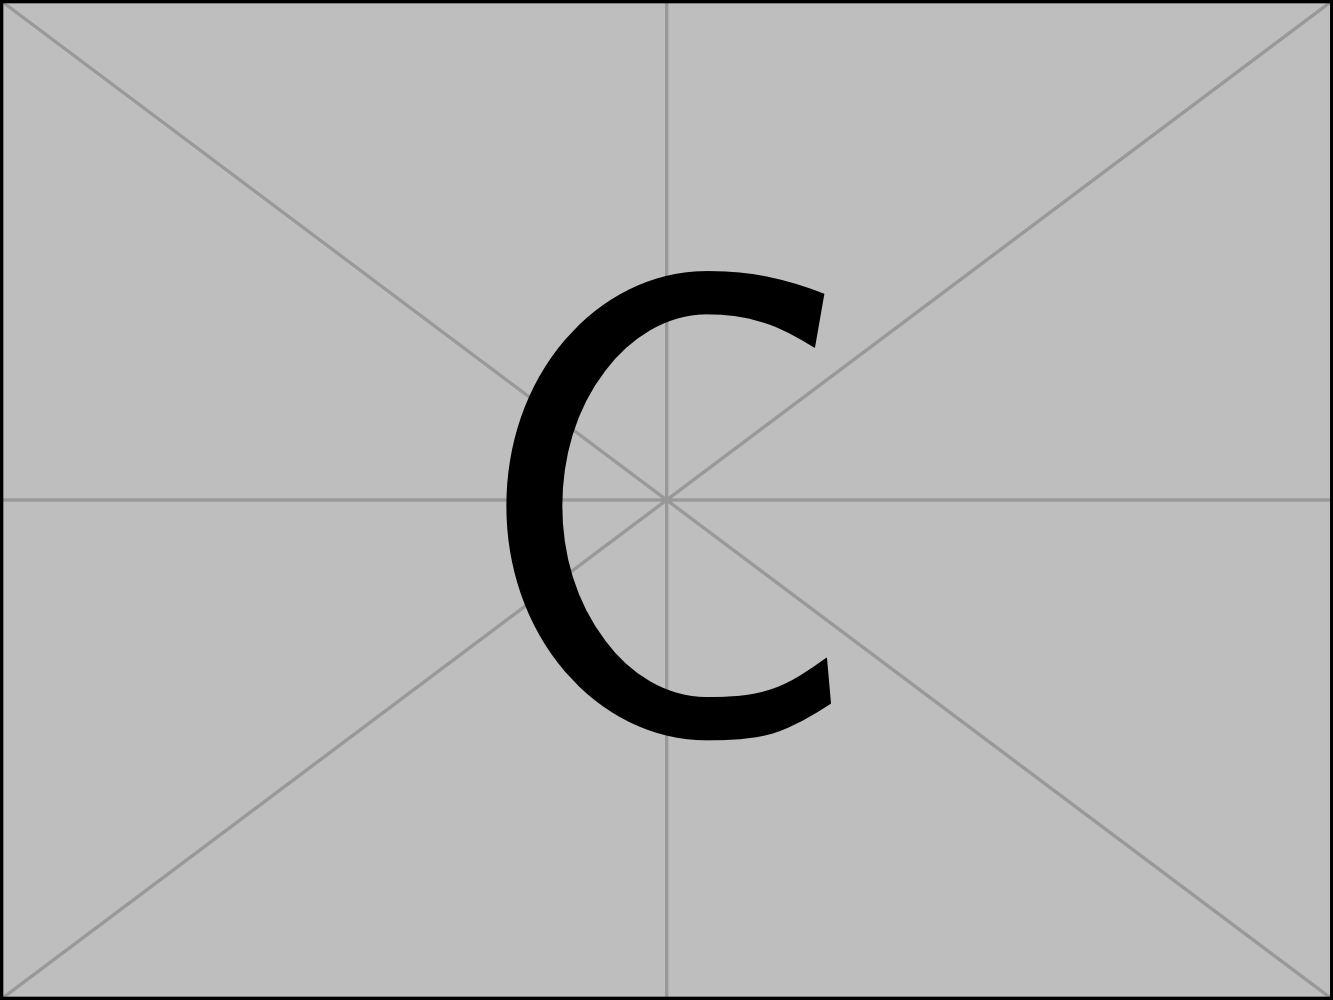
\includegraphics[width=2cm]{fig_image_c.png}} & Protégé contre les corps solides \(\diameter \geq \SI{1}{\milli\meter}\)  	& D	& \adjustbox{valign=t}{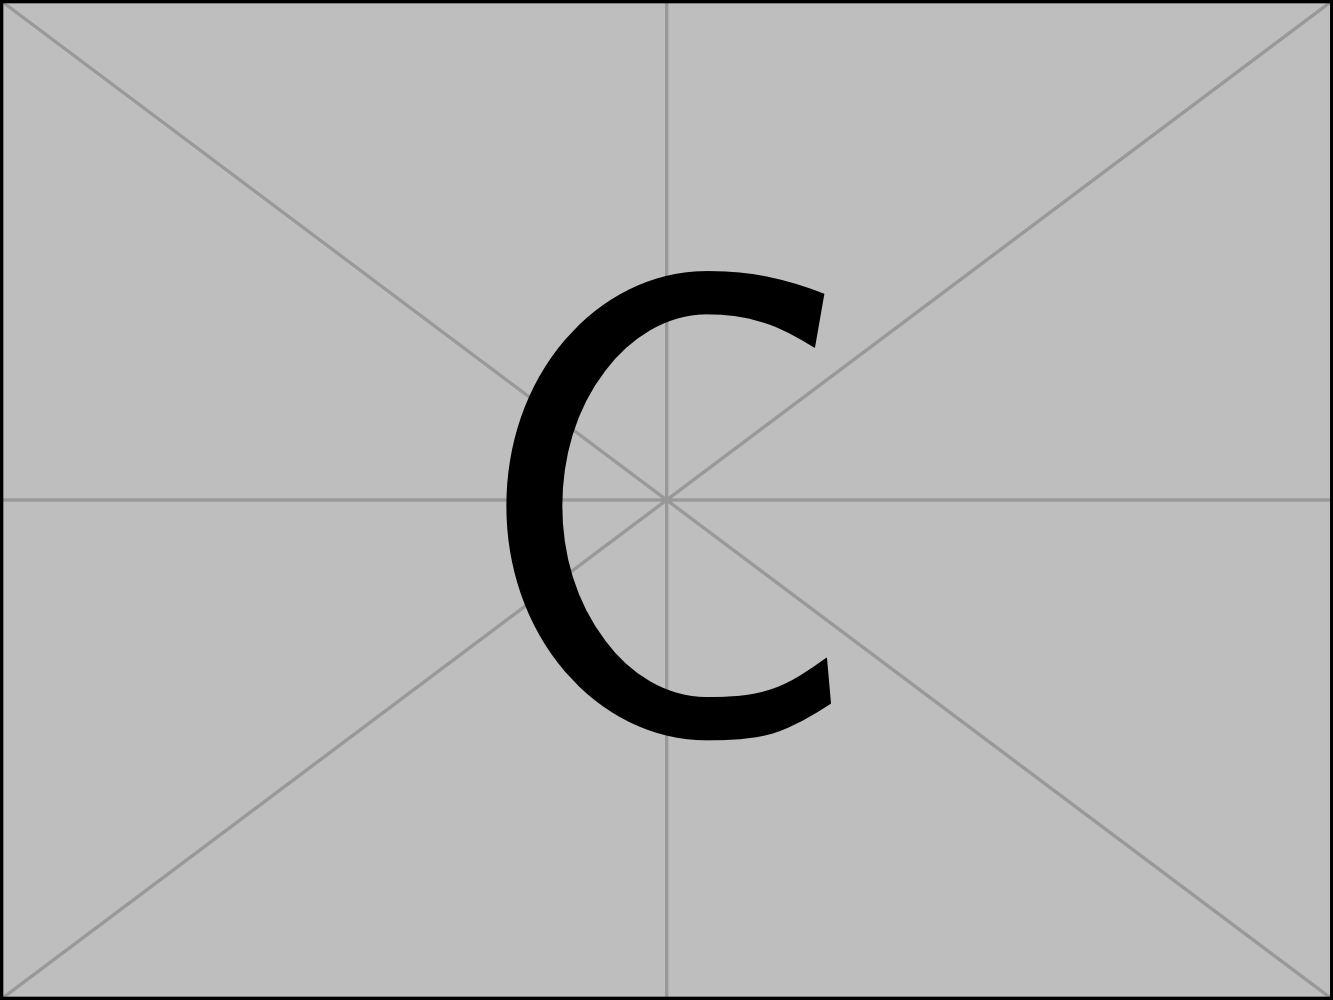
\includegraphics[width=2cm]{fig_image_c.png}}	&	L'introduction d'un outil fin ne permet pas de toucher les parties dangereuses. & 4 & 	\adjustbox{valign=t}{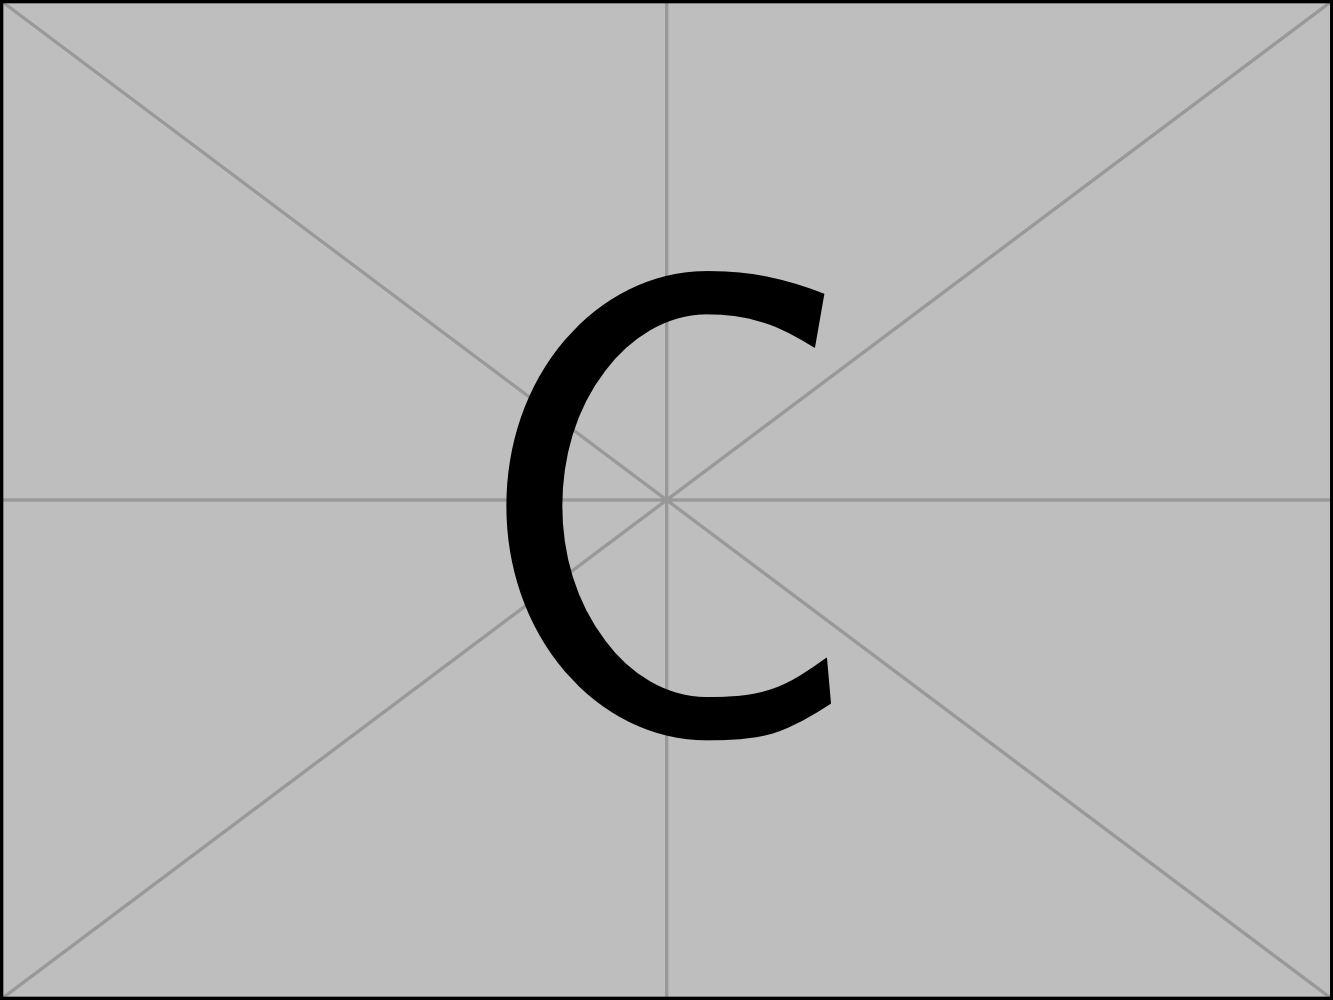
\includegraphics[width=2cm]{fig_image_c.png}}	&	Protégé contre les projections d'eau dans toutes les directions \\
\addlinespace
5 		& 	\adjustbox{valign=t}{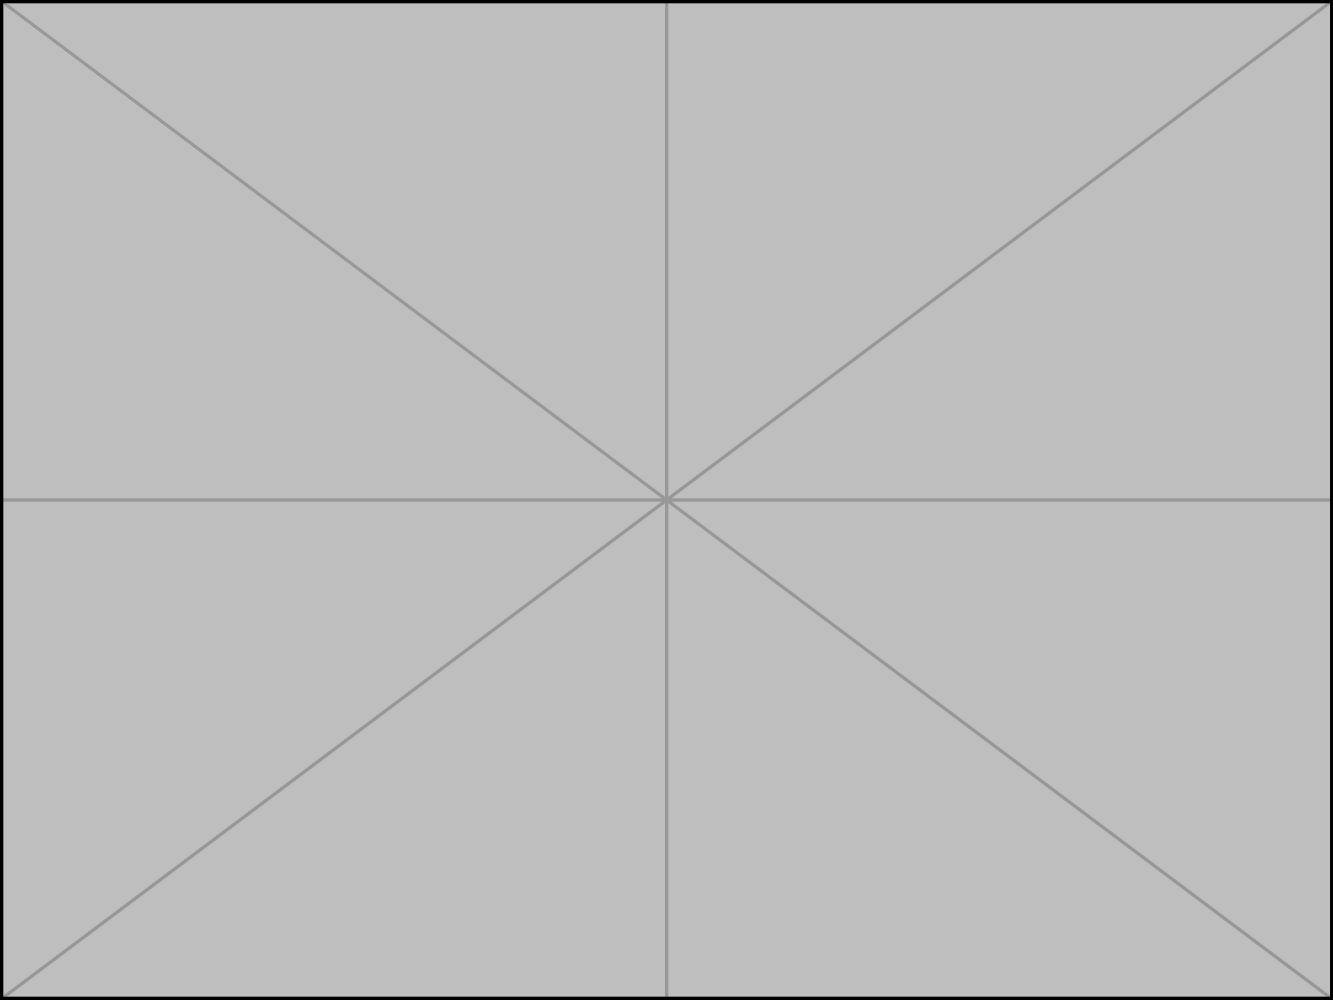
\includegraphics[width=2cm]{fig_image_vide.png}} & Protégé contre la poussière (pas de dépot nuisible)  	& 	& & & 5 & 	\adjustbox{valign=t}{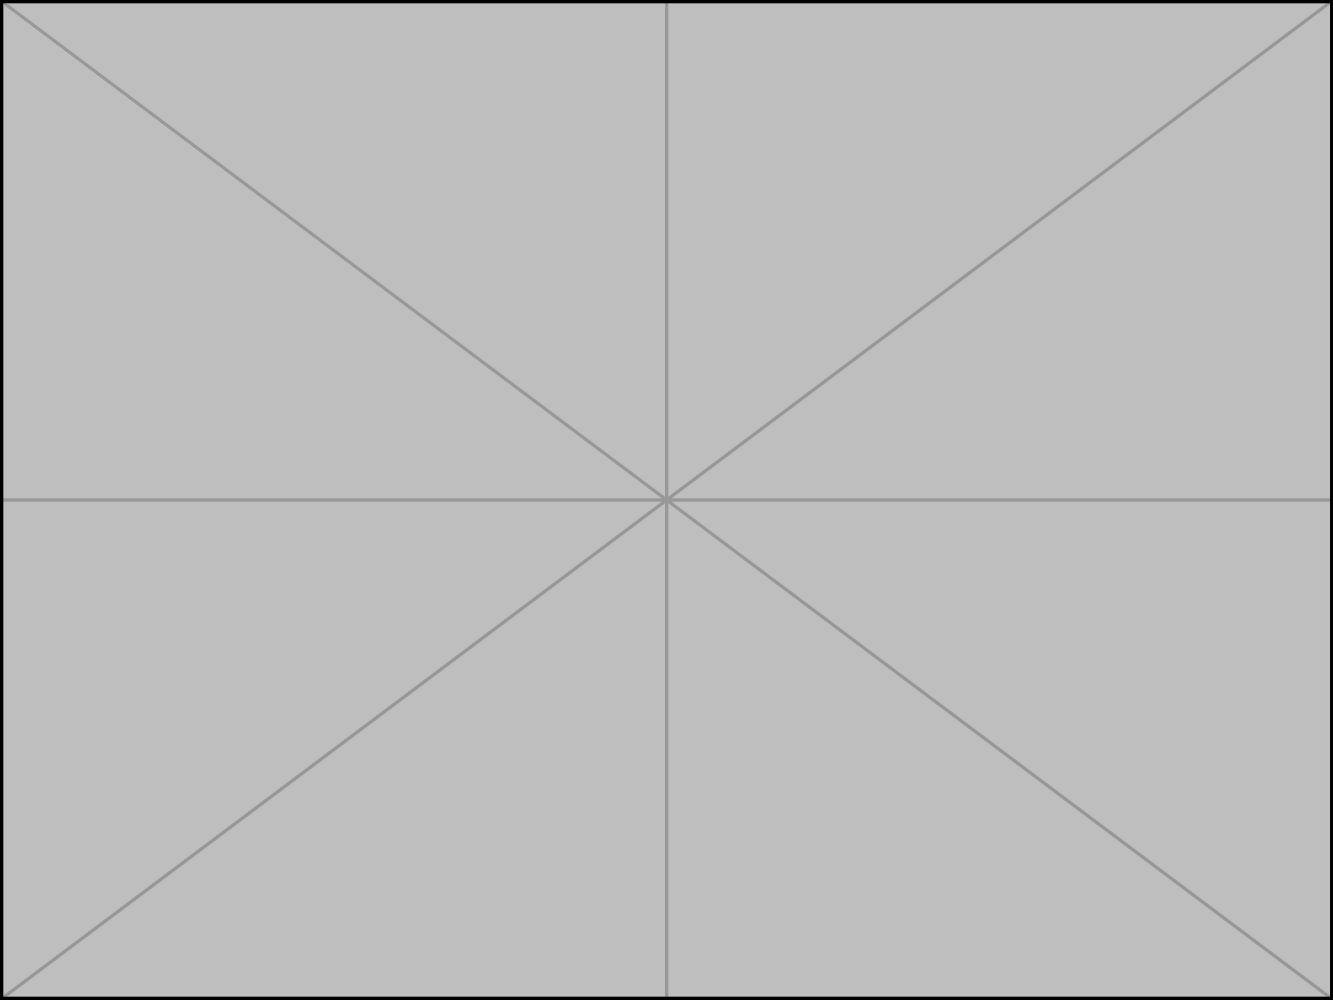
\includegraphics[width=2cm]{fig_image_vide.png}}	&	Protégé contre les jets d'eau dans toutes les directions à la lance \\
\addlinespace
6 		& \adjustbox{valign=t}{
\includegraphics[width=2cm]{fig_image.png}} & Totalement protégé contre la poussière 	& 	& & & 6 & 	\adjustbox{valign=t}{
\includegraphics[width=2cm]{fig_image.png}}	&	Protégé contre les projections d'eau assimilables aux paquets de mer \\
\addlinespace
 		&  & 	& 	& & & 7 & 	\adjustbox{valign=t}{
\includegraphics[width=2cm]{fig_image_a.png}}	&	Protégé contre les effets d'une immersion temporaire dans l'eau \\
 		\addlinespace
		&  & 	& 	& & & 8 & 	\adjustbox{valign=t}{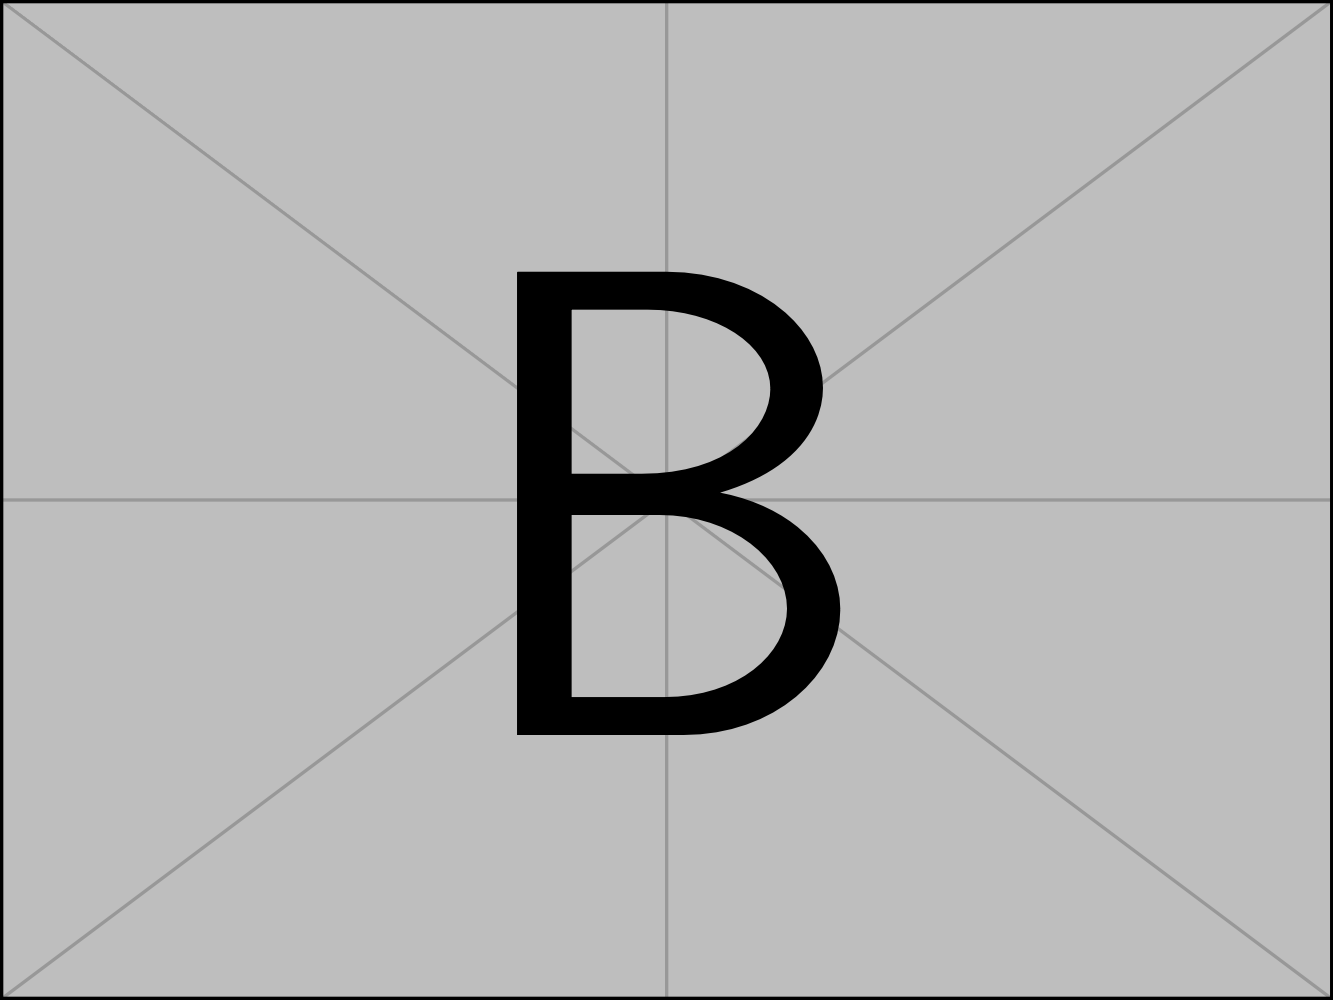
\includegraphics[width=2cm]{fig_image_b.png}}	&	Protégé contre les effets d'une immersion prolongée dans l'eau dans des conditions spécifiées \\
		\addlinespace
		&  & 	& 	& & & 9 & 	&	Protégé contre les jets d'eau haute pression et haute température mais pas nécessairement submersible \\
\end{longtableau}	
  \end{ThreePartTable}

\end{landscape}

\end{document}


